%----------- Terceiro Capítulo: Metodologia --------------

\chapter{Especificação} %(ou especifiação) 10 --- 20 pags

O \emph{software} a ser desenvolvido neste trabalho deverá fornecer uma ferramenta flexível de degradação de vídeo digital e também de avaliação subjetiva e objetiva das mídias.
Neste capítulo serão apresentados os requisitos de tal sistema, assim como as especificações de desenvolvimento, arquitetura e funcionamento.

\section{Análise de Requisitos}

A análise de requisitos é parte fundamental de qualquer projeto, buscando atender da melhor forma as necessidades dos futuros usuários.
Esta sessão descreve os requisitos levantados durante o estudo e planejamento da ferramenta.

\subsection{Requisitos Funcionais}

Requisitos funcionais são aqueles determinados pelas funcionalidades exigidas do sistema, ou seja, as ações que se espera que o sistema execute. 
Foram levantados os seguintes requisitos funcionais:

\begin{itemize}
	\item O \emph{software} deverá possuir ferramentas de degradação de vídeos digitais de blocagem e borramento.
	\item O \emph{software} deverá possuir uma ferramenta de simulação de transmissão \emph{streaming}.
	\item O \emph{software} deverá ser capaz de criar e gerenciar sessões de avaliação subjetiva.
	\item O \emph{software} deverá possuir uma ferramenta que realize avaliação objetiva sobre os vídeos da base de dados, conforme as métricas PSNR, MSE e MSSIM.
	\item O \emph{software} deverá ser capaz de exibir os vídeos existentes na base de dados.
	\item O \emph{software} deverá exibir os resultados das avaliações objetivas e subjetivas de forma gráfica.
\end{itemize}

\subsection{Requisitos Não-Funcionais}
\label{met:reqnaofunc}

Requisitos não-funcionais são aqueles ditados por restrições ou exigências de qualidade ou de operação, tais como performance, segurança ou tecnologias envolvidas.
Abaixo se encontram os requisitos não funcionais levantados:

% TODO dividir por categorias: padronização, usabilidade, tecnologias envolvidas.

\begin{itemize}
	\item As ferramentas de degradação e métricas objetivas deverão operar sobre vídeos em formato YUV planificado com subamostragem 4:2:0.
	\item A ferramenta de simulação deverá operar sobre vídeos no formato \sigla{H.262}{Padrão de compressão de vídeo digital também conhecido MPEG-2 Part 2} encapsulados em um \emph{Transport Stream} (\sigla{TS}{Transport Stream}).
	\item O sistema deve fornecer documentação detalhada de auxílio ao uso das ferramentas.
	\item A ferramenta de exibição deverá ser executada em um sistema capaz de prover um \emph{display} com resolução igual ou maior que a dos vídeos a serem exibidos.
	\item A interface gráfica do sistema necessita que haja um \emph{Java Runtime Environment} (\sigla{JRE}{Java Runtime Environment}) instalado no sistema operacional.
	\item O \emph{player} de vídeo MPlayer, livre e de código aberto, é necessário para mostrar os vídeos durante as sessões.
	\item O projeto deverá ser desenvolvido utilizando ferramentas de distribuição livre.
	\item O \emph{software} deve ser capaz de operar independentemente do SGBD utilizado.
	\item O sistema deve ter um tempo de resposta adequado, de forma que este não interfira no \emph{timing} das avaliações subjetivas.
	\item As ferramentas desenvolvidas devem estar disponíveis independentemente do sistema (\emph{stand-alone}).
\end{itemize}

\section{Especificações do Software}

Esta seção tem o propósito de descrever a arquitetura proposta para o SASQV2, assim como abordar as diferentes linguagens e bibliotecas que ajudam a integrar o programa.

\subsection{Arquitetura do Sistema}

Por se tratar da continuação do desenvolvimento do projeto SASQV, este trabalho reutiliza e adapta grande parte dos componentes existentes no trabalho original.

A Figura \ref{fig:arquitetura} mostra uma comparação entre as visões gerais de ambos os projetos. A diferença mais notável entre estas arquiteturas é a separação dos componentes de serviço e o de ferramentas, além de também recriar o componente de interface gráfica para melhor atender às necessidades do sistema.

Mais detalhes sobre cada componente da arquitetura são descritos em seções específicas a seguir.

\begin{figure}[!htb]
	\centering
	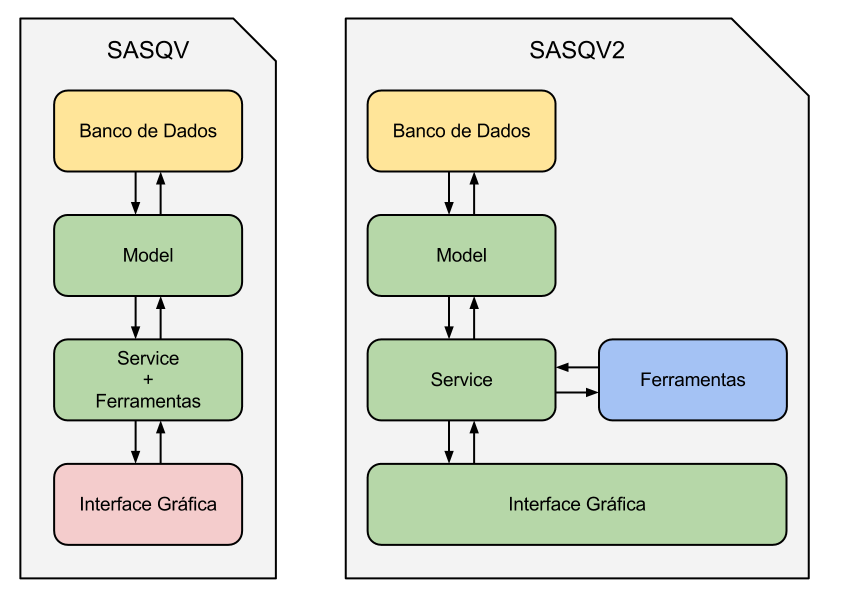
\includegraphics[width=0.9\textwidth]{./imgs/arquitetura.png}
	\caption{Visão geral das arquiteturas dos sistemas SASQV e SASQV2.}
	\label{fig:arquitetura}
	\fonte{Autoria Própria.}
\end{figure}

\subsubsection{Banco de Dados}

O componente banco de dados foi completamente reaproveitado, seguindo as mesma especificações do SASQV.

O Sistema Gerenciador de Banco de Dados (\sigla{SGBD}{Sistema Gerenciador de Banco de Dados}) escolhido foi o MySQL, atualmente o SGDB \emph{open source} mais utilizado no mundo \cite{mysqlmarket}.
O MySQL foi lançado e desenvolvido em 1995 pela empresa Sueca MySQL AB, atualmente incorporada pela Oracle Corporation, na forma de um SGDB que fornece um servidor multi-usuários para bancos de dados relacionais \cite{wikipediamysql}.

Juntamente do MySQL também é utilizado o MySQL Workbench, uma ferramenta distribuída pela Oracle que concilia um cliente MySQL, uma ferramenta de \emph{Database Moddeling} e um administrador de servidor MySQL.
A versão \emph{open source} de ambas as ferramentas é distribuída sob a licensa GNU General Public License (\sigla{GPL}{General Public License}).

O modelo Entidade-Relacionamento (\sigla{ER}{Entidade-Relacionamento}) é o mesmo utilizado pelo SASQV, como mostrado na Figura \ref{fig:diagramaER}.

\begin{figure}[!htb]
	\centering
	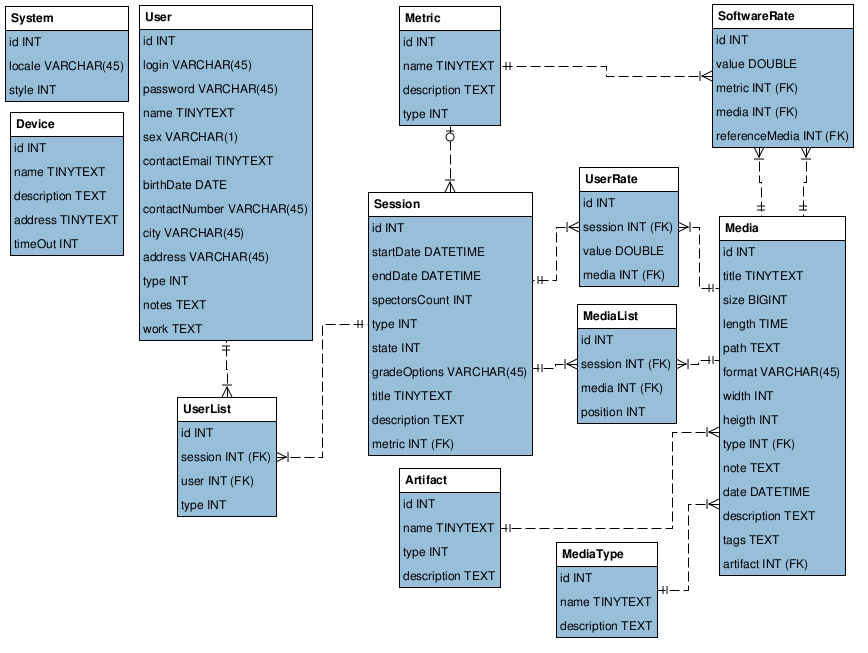
\includegraphics[width=0.9\textwidth]{./imgs/diagramaER.png}
	\caption{Diagrama Entidade-Relacionamento do SASQV2}
	\label{fig:diagramaER}
	\fonte{Autoria Própria}
\end{figure}

\subsubsection{Model}

O componente Model presente no SASQV2 também foi inteiramente reaproveitado do SASQV, cabendo apenas algumas adições. Este componente consiste na implementação de um mapeamento objeto-relacional (\sigla{MOR}{Mapeamento Objeto Relacional}) por meio da biblioteca Hibernate.

O Hibernate teve seu desenvolvimento iniciado em 2001 por Gavin King, com o objetivo de melhorar as ferramentas de persistência existentes na plataforma Java \cite{hibernateHistory}, e é atualmente distribuído sob a licensa GNU Lesser General Public License (\sigla{LGPL}{Lesser General Public License}) \cite{hibernateAbout}.

A biblioteca provê um mapeamento flexível entre objetos Java e tipos SQL, eliminando a custosa necessidade de processamento manual e repetitivo de listas de resultados obtidas via SQL e JDBC.
Estima-se que até cerca de 30\% do código de uma aplicação possa ser poupado utilizando MOR, além de incrementar a portabilidade do sistema suportando diversas implementações de Bancos de Dados SQL em troca de um pequeno \emph{overhead} de performance.

\subsubsection{Service}

Este elemento também foi reaproveitado, no entanto sofreu diversas adaptações em sua estrutura para comportar novas funcionalidades e continuar suportando as antigas.
O componente presente no SASQV se trata de uma fachada de serviço responsável por interpretar mensagens provenientes da interface e distribuí-las em uma das três formas a seguir:

\begin{enumerate}
	\item Executar uma ação de degradação ou métrica objetiva.
	\item Repassar uma ação para o dispositivo sem-fio e esperar por resposta.
	\item Repassar uma ação para o elemento model e esperar por resposta.
\end{enumerate}

Na arquitetura do SASQV2 a interpretação de mensagens foi descartada, uma vez que foi prosposta a implementação de uma nova interface em linguagem Java, que deu lugar a métodos de finalidades distintas dentro de cada ação enumerada acima. 
Com isso a execução de tarefas de degradação ou avaliação por métrica objetiva, antes executadas localmente, passaram a ser delegadas para um novo componente chamado Ferramentas, descrito em \ref{met:ferramentas}.

Já o conteúdo dos métodos que repassam as ações para o dispositivo sem-fio e para o model permanecem muito semelhantes aos encontrados na interpretação de mensagens originalmente feito no SASQV, sofrendo apenas pequenas modificações para acomodar a nova estrutura.

\subsubsection{Ferramentas}
\label{met:ferramentas}

O módulo ferramentas constitui um novo componente na arquitetura do \emph{software}, visto que um dos objetivos deste trabalho é desenvolver melhores ferramentas de degradação considerou-se válida a separação deste módulo que originalmente se encontrava juntamente do Service.

Esse módulo é resposável por todas as ferramentas que de alguma forma manipulam vídeos digitais ou auxilíam nesta manipulação. Dessa forma foram desenvolvidas 5 ferramentas distintas, em linguagem C++:

\begin{description}
	\item[Block] Cria o efeito de blocagem nos vídeos.
	\item[Blur] Cria o efeito de embaçamento nos vídeos.
	\item[Netsim] Efetua uma simulação de streaming de vídeo digital com perda informação.
	\item[Raffle] Ferramenta auxíliar para distribuição temporal e espacial dos artefatos.
	\item[Metric] Efetua avaliação dos vídeos por meio de métricas objetivas.
\end{description}

Estas ferramentas podem receber configurações independentes e flexíveis, diversificando as possibilidades de geração de degradações e artefatos e tornando possível a criação de resultados diferenciados para um mesmo vídeo usado como referência. Dentre essas configurações pode-se destacar a distribuição dos artefatos no tempo e no espaço e a intensidade de aplicação dos mesmos. Cada ferramenta citada será descrita com mais detalhes em \ref{des:ferramentas}. 
A independência das ferramentas permite a utilização combinada em sequência, de forma que a cada utilização é possível aplicar artefatos à videos originais ou já degradados, criando inúmeras combinações de degradação. A figura \ref{fig:fluxogramaferramentas} demonstra o fluxo de utilização das ferramentas em conjunto com uma base de vídeos.

\begin{figure}[!htb]
	\centering
	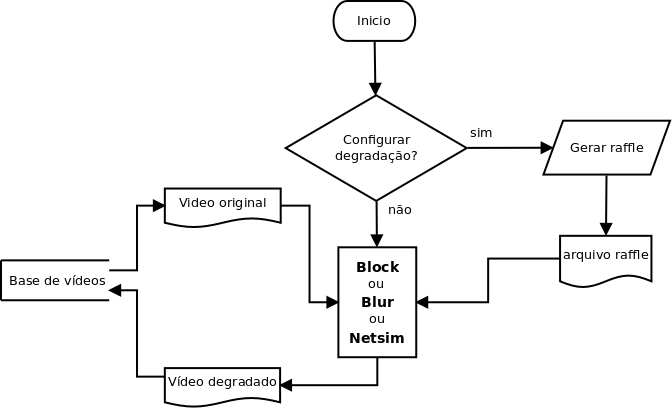
\includegraphics[width=0.9\textwidth]{./diagramas/fluxodegradacao.png}
	\caption{Fluxograma de utilização das ferramentas.}
	\label{fig:fluxogramaferramentas}
	\fonte{Autoria Própria}
\end{figure}

\subsubsection{Interface Gráfica}

Originalmente desenvolvida utilizando a tecnologia Adobe Flex, era necessária a utilização de uma biblioteca exclusivamente para comunicação entre os módulos de Interface e Service. A biblioteca utilizada (merapi) se encontrava em fase de desenvolvimento beta e carecia de funcionalidades, de forma que seria necessário buscar uma biblioteca alternativa para continuar o densevolvimento do projeto.

Além disso, as ferramentas de desenvolvimento em tecnologia Flex não são gratuitas e perderam gradativamente o suporte à sistemas operacionais Linux.

A combinação destes fatores motivou a decisão de desenvolver uma nova intercae Gráfica utilizando Java, proporcionando melhor integração, reduzindo o envolvimento de diversas tecnologias e bibliotecas e assim aumentando a portabilidade da ferramenta.

\subsection{Linguagens}

Por se tratar da aprimoração e continuação do projeto SASQV a primeira linguagem contemplada foi a presente no mesmo: Java.

Esta foi desenvolvida por uma equipe de programadores liderada por James Gosling, trabalhando para a empresa Sun MicroSystems \cite{wikijava}. Sendo lançada em 1995, era o principal componente da plataforma Java e demonstrava forte inspiração na linguagem C++, compartilhando parte de sua sintaxe e também diversas característica.

No entanto, Java é considerada uma linguagem de mais alto nível, além de ser compilada no formato \emph{bytecode}, o que favorece a portabilidade dos programas, podendo ser executados em diversas arquiteturas e sistemas operacionais, contanto que estes possuam uma implementação da Java Virtual Machine (\sigla{JVM}{Java Virtual Machine}). Uma das facilidades da linguagem é a sua extensa biblioteca padrão, que contém, entre outros, diversos componentes para construção de interfaces gráficas.

A linguagem C++ também passou a ser considerada para o desenvolvimento do projeto, visto o desenvolvimento do módulo de Ferramentas como programas que possam ser usados independentemente.
A linguagem teve seu desenvolvimento iniciado por Bjarne Stroustrup em 1979, quando trabalhava na Bell Labs \cite{wikicplusplus}.
C++ é uma nova implementação da linguagem C adicionada de novas funcionalidades, tais como suporte a classes, sobrecarga de operadores, herança múltipla e tratamento de exceções.
Atualmente, C++ é uma das linguagens mais populares, sendo implementada em diversas plataformas de \emph{hardware} e sistemas operacionais, além de ser usada na implemantação dos mais diversos \emph{softwares} para \emph{desktop}, \emph{drivers} de dispositivos de \emph{hardware} e sistemas embarcados.

Um dos principais atrativos da linguagem para o desenvolvimento das ferramentas deste projeto é a existência de diversas funcionalidades de baixo nível.
Essas funcionalidades simplificam e facilitam o acesso e manipulação \emph{byte} a \emph{byte} de \emph{streams} de dados, algo que é usado extensivamente ao longo da implementação das ferramentas.
Outro aspecto importante derivado destas funcionalidades é o impacto na performance do software. 
Segundo \cite{benchmarks}, para o \emph{benchmark reverse-complement} --- onde são efetuadas diversas operações de leitura e escrita em arquivos, além de um leve processamento --- a melhor implementação em Java foi 1.9 vezes mais lenta que a melhor implementação em C++.
A simplicidade da linguagem também facilita o desenvolvimento de ferramentas \emph{stand-alone} com interface por linhas de comando, além de possuir diversas bibliotecas de \emph{parsing} para comandos e opções.

Ambas as linguagens eram previamente conhecidas pelos integrantes do projeto, os quais também possuem um nível confortável de experiência no desenvolvimento de aplicações com estas linguagems e com diversas ferramentas associadas a elas, como IDE's, bibliotecas gráficas e conectividade com bancos de dados.

\subsection{Diagramas de Caso de Uso}

Uma das primeiras fases em um projeto de \emph{software} é a construção de diagramas de Casos de Uso. Estes diagramas auxiliam no processo de levantamento de requisitos e de entidades que deverão interagir com o sistema. Também auxiliam na definição e visualização dos serviços a serem desempenhados pelo sistema.

Os casos de uso elaborados foram divididos em diferentes diagramas, dando enfoque as funcionalidades mais importantes a serem desempenhadas pelo \emph{software}: degradar vídeos, realizar avaliação objetiva e realizar avaliação subjetiva através da criação de uma sessão de vídeos.

O diagrama apresentado na Figura \ref{fig:ucdgeral} mostra o caso de uso geral. Para que o usuário possa interagir com o sistema é necessário realizar \emph{login} no sistema utilizando usuário e senha válidos. Esta validação é realizada pelo \sigla{SGBD}{Sistema Gerenciador de Banco de Dados} (Sistema Gerenciador de Banco de Dados), representado no diagrama pelo ator de mesmo nome.

O sistema SASQV original previa a existência de dois tipos de ator: administrador e avaliador. O primeiro possuía permissões para acessar o sistema e realizar todas as operações, menos realizar avaliações de vídeo. O segundo, ao contrário do primeiro, só poderia realizar avaliações. Em prol da simplicidade, optou-se por permitir que avaliadores também pudessem realizar as mesmas ações que o administrador, sendo necessário apenas um destes atores.

Concluído o \emph{login}, o usuário pode realizar atividades como criar uma sessão para avaliação subjetiva; degradar vídeos; adicionar ou remover vídeos da base de dados; adicionar, remover ou editar cadastro de usuários; consultar resultados através de gráficos; consultar tópicos de ajuda; realizar avaliações objetivas utilizando as ferramentas desejadas e, por fim, modificar configurações gerais do sistema.

\begin{figure}[!htb]
	\centering
	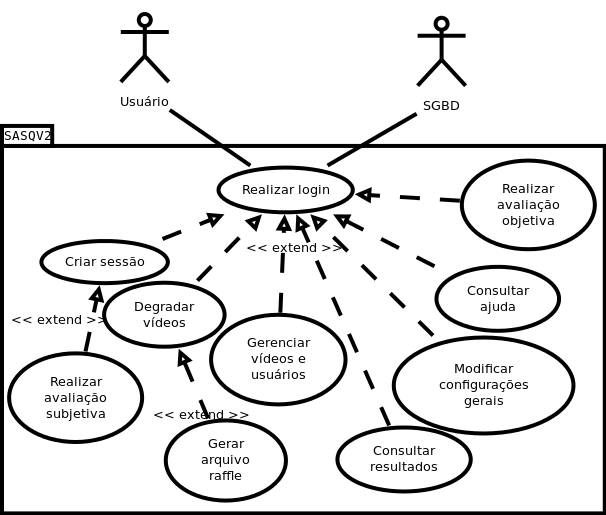
\includegraphics[width=0.9\textwidth]{./diagramas/casodeuso2.png}
	\caption{Geral.}
	\label{fig:ucdgeral}
	\fonte{Autoria Própria}
\end{figure}

Uma das funcionalidades mais importantes do sistema proposto é a realização de sessões para avaliação subjetiva. Para criar uma sessão, primeiramente é necessário definir a identificação assim como os parâmetros de configuração. O próximo passo é a escolha dos vídeos da base de dados que serão apresentados. Por fim, são selecionados os equipamentos que serão utilizados. Todos os passos interagem com o SGBD, seja realizando consultas, seja atualizando-o.

\begin{figure}[!htb]
	\centering
	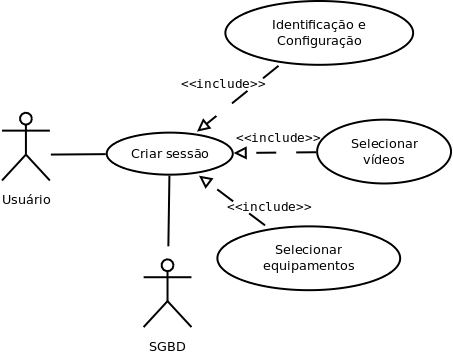
\includegraphics[width=0.9\textwidth]{./diagramas/sessao.png}
	\caption{Sessão.}
	\label{fig:ucdsessao}
	\fonte{Autoria Própria}
\end{figure}

O próximo diagrama, na Figura \ref{fig:ucddegradacao}, apresenta duas funcionalidades do sistema: degradar vídeos e realizar avaliação objetiva. A degradação de vídeos depende da seleção dos vídeos desejados e da seleção da degradação a ser aplicada, conforme os parâmetros informados. Para realizar uma avaliação objetiva, basta selecionar os vídeos e métricas desejadas.

\begin{figure}[!htb]
	\centering
	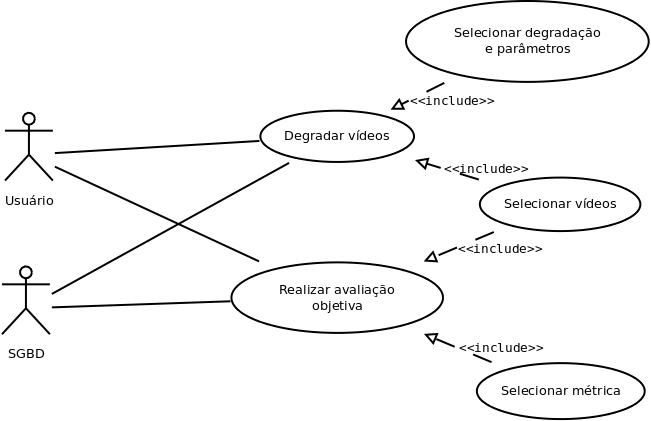
\includegraphics[width=0.9\textwidth]{./diagramas/degradacao.png}
	\caption{Degradação.}
	\label{fig:ucddegradacao}
	\fonte{Autoria Própria}
\end{figure}

\section{Considerações}

Para este projeto de \emph{software} procurou-se aproveitar ao máximo os componentes existentes no SASQV, de forma a maximizar o esforço nos aspectos a serem melhorados e não consumir tempo de projeto retrabalando o que já foi feito. 

A adesão ao desenho de \emph{software} apresentado se justifica pela independência entre os componentes, facilitando o desenvolvimento e teste de cada um e também o reaproveitamento em trabalhos futuros.
A opção por criar ferramentas independentes para o processo de degradação se mostra eficiente e versátil, visto que deste modo estão prontas para serem reutilizadas e combinadas à outras ferramentas, além de facilitarem a automatização do processo de degradação para o usuário avançado.

Sendo assim, a estrutura planejada foi muito semelhante à do projeto original, com diversos componentes sofrendo adaptações e também a adição de um novo componente dedicado.
